 \chapter{Introduction}
\label{chapter:introduction}

Artificial Intelligence has proved itself to be a useful approach for tools in the field of \textbf{Computer Aided Diagnosis (CID)}. Modern \textbf{Computer Vision (CV)} approaches, powered by the \textbf{Deep Learning (DL)} \cite{lecun2015deep} paradigm resulted in impressive advancements in Digital Image Processing. Researchers were quick in proposing methods able to autonomously analyze and diagnosis patients based on medical images including CT scans and MRIs.

As hardware further developed and adapted in order to support computationally expensive deep learning models another type of medical image was approached. Although previously unfeasible to processes, histological images encapsulate valuable information which can be employed to diagnose infections, cancers and various other diseases which are invisible in any other medical data. 

In Histopathology, the diagnosis takes place based on the most basic building blocks of the human body : cells and tissue. Images are obtained through microscopes and have huge dimensions which are sometimes larger than 100,000 x 100,000 pixels. Furthermore, histological images can be captured using various magnification factors increasing the complexity of any problem from the field. The next illustration, \textbf{Figure \ref{histo_img}} showcases an example of such histological images.

\begin{figure}[htb]
    \centering
	\centerline{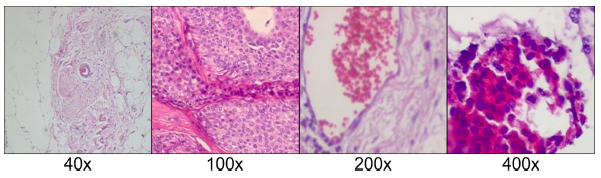
\includegraphics[scale=1]{figures/breast_histoimg_multiple_scales.png}}
	\caption{Example of histological images, captured at multiple magnification factors. Image from \cite{bayramoglu2016deep}}
	\label{histo_img}
\end{figure}

Due to the characteristics of these images, annotation in this field remains extremely expensive. Even a single sample requires many work hours from a trained expert, usually a doctor. Although not as costly as annotation, diagnosis also requires notable effort thus automating this process through the use of intelligent methods has the potential to streamline a process which affect millions of patients and non-patients. 

Fully automated systems in this field would allow people to get regular checks at a low price. This is essential in combating diseases like cancer in which early diagnosis drastically increases the survival rate. The promise of such a model encouraged researchers to develop various datasets focused on different organs and their organs including: liver, prostate, colon and breasts.

One class of Deep Learning models which recently obtained impressive results in multiple histopathology Computer-aided Diagnosis problems are \textbf{Multi-task (MT)} models. The benefits of the Multi-task Learning \textbf{(MTL)} paradigm \cite{caruana1997multitask} are manifold. First of all, this type of approach usually results in algorithms with better generalization. Secondly, as a single sample may be used for two predictions, some components of the network, such as encoders, are able to exploit this increased data efficiency and achieve faster model convergence. Moreover, training a single Multi-task network requires less computational resources when compared with the prospect of training two independent networks. 

All these desirable qualities make Multi-task models well suited for intelligent applications in Medicine, especially in Digital Histopathology where sample scarcity and massive image dimensions encourages the maximization of data efficiency and the reduction of the computational cost. 

The aim of this work is to analyse recent approaches from the Digital Histopathology field which employ Deep Multi-task models and identify possible future research directions. The rest of this report is structured in the following manner. In \textbf{Chapter \ref{chapter:RelatedWork}} Deep Multi-task models are introduced. Next, \textbf{Chapter \ref{chapter:InvestigatedApproach}} analyses recent MT approaches applied in various histopathology problems. The advantages and limitations of the previously mentioned methods are discussed in \textbf{Chapter \ref{chapter:Discussion}}. Lastly, \textbf{Chapter \ref{chapter:5-Conclusions}} concludes the report.